
\documentclass[12pt, oneside]{amsart}
\usepackage[parfill]{parskip}
\usepackage{graphicx}
\usepackage{amssymb}
\usepackage{epstopdf}
\usepackage{url}
\usepackage[comma,authoryear]{natbib}
\usepackage{setspace}

\doublespacing
\DeclareGraphicsRule{.tif}{png}{.png}{`convert #1 `dirname #1`/`basename #1 .tif`.png}
\DeclareMathOperator*{\argmax}{arg\,max}

\title{Management of the Distributed Fishery Commons}
\author{James Rising}

\begin{document}
\maketitle

\begin{singlespace}
{\it Below I sketch the main points of inquiry for a new model of commons applied to fisheries management, along with the model's implications for the political economy surrounding local stakeholders, governing institutions, and their cross-scale interactions.  There may be an extensive body of research on this or a similar model; I do not know, and I have not yet been able to discover it (but I haven't spent much time looking for it yet).  My final paper would expand on these points and better locate the ideas in existing research.}
\end{singlespace}

This paper develops the concept of the ``distributed commons'' in the context of fisheries management.  A distributed commons differs from an normal commons in that both the boundaries of the system are imprecise and the situation within the commons is significantly affected by dynamics outside of it.  This conception brings to the fore the role of perspective and scale (including cross-scale aspects) in understanding the political economy of management.  In the first section, a general theory of distributed commons is developed.  In the section section, the consequences of this theory are explored for one aspect of fisheries management: the capacity for local fishing communities to encourage overarching regulatory regimes that then support their ability to self-organize sustainable fisheries.

Fishery collapse is a global concern, affecting world food supply, economic prospects for fishing communities, and with plenty of spill-over effects for marine environments and endangered species. A growing set of policies are available address this problem, including catch quotas, gear restrictions, marine reserves, and community management.  However, a variety of systemic problems have continued to hamper these policies, including entrenched stakeholders, mistrust of science, uncertainties in fish stocks, decisions oriented toward short-term gains, questions of sovereignty, extreme subsides, and incentives to hide catches.

Despite aspects which are normally taken to be barriers to community management, including migratory stocks, ambiguous spatial boundaries, and weak state support, some regions have had considerable success \citep{pinho2012overcoming}.  This research concentrates on commons that share these characteristics and asks how further success might be possible.

\section*{The Distributed Commons}

% PART 1
% General theory of distributed commons, examples from fisheries

A distributed commons is a kind of open commons, a non-excludable, rivalrous resource.  While commons are typically conceived of as an elemental source of goods, like a village green available for sheep grazing, many of the resources subject to the tragedy of the commons and of widespread concern today are more distributed.  For example, fish stocks, timber, groundwater, and other ecosystem services are exploited and impacted differently through space, where the relevant stakeholders vary.  Modeling and thinking about these resources in a non-distributed and non-spatial can significantly distort our understanding of the system and our choices within it \citep{durrett1994importance}.

This distinction is most relevant when considering scale issues.  At either a local or a region scale, a distributed commons-- for example, a fishing area-- is a commons with an ambiguous boundary and an open community of users.  As with any commons, anyone in the community can access it for individual benefits, with the potential for (a) aggregate externalities and (b) collective or autocratic management.  Classic commons theory presumes that both the scope of the resource and the community with the potential to access it are clearly and completely defined.

These assumptions are modified for distributed commons.  There is no clear boundary defining a scope of the commons relevant to a given stakeholder, and different stakeholders may have very different views of the resources available and community using it.  Property, a central question for classic commons, becomes less relevant.  One's capacity to lay claim to a parcel of the greater commons is easier than to ensure that activities beyond that parcel do not impact one.

On the other hand, management options only need to apply to a region.  The necessary size of that region depends on the properties of the underlying resource.  For example, management of tuna may require rules over oceans since tuna are so mobile, while forest management may need only small buffer zones.

Sinks and sources are important factors in distributed commons.  For example, Marine Protected Areas can act as sources of fish in otherwise unmanaged fisheries, greatly increasing their sustainability \citep{gell2003benefits}.  A commons is overexploited when the sinks in a given region exceed the sources, and the degree of exploitation can differ in space.

A distributed commons is best analyzed from the perspective of a particular stakeholder.  The scale on which that stakeholder operates-- for example, a boat and a fishing area-- define a local scale.  At that local scale and in the region of the central stakeholder, an array of other users coexist, cooperate, and compete.  In addition, other users at a local scale but in more distant regions may affect the conditions in the stakeholder's region.  These might be called ``outsiders'', for example in the case of international commercial fishers who now fish off the coasts of Africa [ref].  The institutions that span the region of the central stakeholder operate on a regional scale.  For fisheries, these include the governing bodies that impose management policies, and have grown to span multiple fisheries.

% boundaries of system imprecise both because no clear border, because system is open, and because knowledge of fisheries currently has much uncertainty and is evolving.

\section*{Conceptual Model of the Distributed Commons}

Diagram 2-a of figure \ref{fig:diagrams} shows a model of a distributed commons.  In contrast to a classic commons, where it is exactly the capacity for multiple users to simultaneously use a resource that is its defining feature and the source of its problems, the distributed commons is conceptually segmented into parcels under exploitation by at most one user.  These parcels may fluidly shift in size and physical location, but it is not their simultaneous use that causes problems.  Instead, the tragedy of the commons results from the aggregate drain of many localized sinks.  That tragedy may only apply to a region, or may be felt across the entire distributed commons.  The aggregate problems comes from cross-boundary effects and the movement of critical elements between between the parcels.  These elements may be the actual resource (e.g., fish in the case of resource stocks), a necessary input (e.g., water for agriculture), or ecosystem services which rely on a wider domain (e.g., bee pollination services).

For many real commons, this makes natural sense.  The space that a boat physically occupies is excludable.  For groundwater use, each well occupies a distinct column, but too many wells across a region cause overuse.

\begin{figure}[htp]
  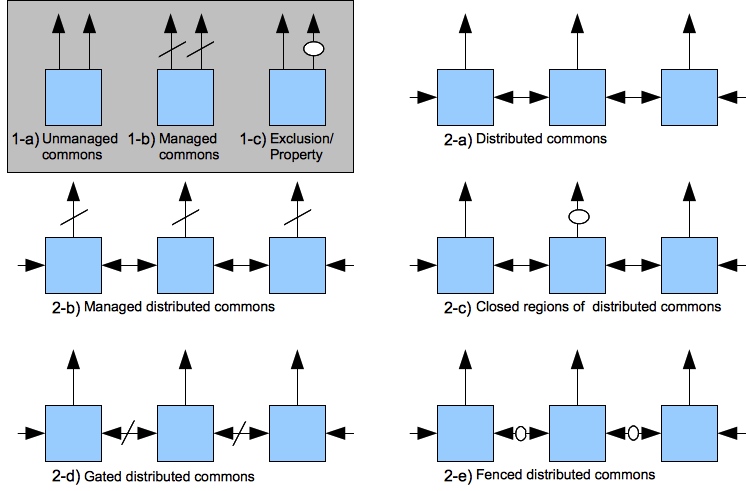
\includegraphics[width=6.5in]{diagrams.png}
  \caption{Classes of governance options for distributed commons.  The boxed schemas denote the classic commons; the rest show a general model for the distributed commons and classes of management options for it.  See text for descriptions.}
  \label{fig:diagrams}
\end{figure}

The diagrams in figure \ref{fig:diagrams} explore some basic classes of management strategy available for commons, at the regional scale.  Within classic common, three general options are as follows.

\begin{description}
  \item[Unmanaged commons (1-a)]
    A classic commons, with multiple users exploiting it simultaneously.
  \item[Managed commons (1-b)]
    The exploitation of all users of the resource is limited in a way that requires monitoring.
  \item[Exclusion/property (1-c)]
    The tragedy of the commons is resolved by enforcing property rights, excluding all but a single or self-managing community of users.
\end{description}

For distributed commons, the same abstract approaches yield more options, due to the greater complexity of the model.

\begin{description}
  \item[Distributed commons (2-a)]
    Rather than imagining multiple users of one area, each area is exploited by at most user.
  \item[Managed distributed commons (2-b)]
    All users within a region are managed, through limiting and monitoring.
  \item[Closed regions of distributed commons (2-c)]
    Some regions can be closed, providing sources to offset sinks elsewhere.
  \item[Gated distributed commons (2-d)]
    The flow of materials between parcels (or equivalently, the material sizes of each parcel) can be monitored and impeded.
  \item[Fenced distributed commons (2-e)]
    The flow of materials between parcels (or equivalently, their material sizes), can be shut off, so that each parcel acts like a classic commons.
\end{description}

The diagram shows the distributed commons modeled on along a line, appropriate for a coast, but a grid or network would better represent spatial regions.  A network could also be used to represent nutrient flows through more complicated food webs, with multiple interacting resource systems.

Methods for studying groundwater levels provide an simplified model for some of the interaction scenarios that are possible.  Figure \ref{fig:capacity} combines stock level graphs with yield graphs for the central stakeholder.

\begin{figure}[htp]
  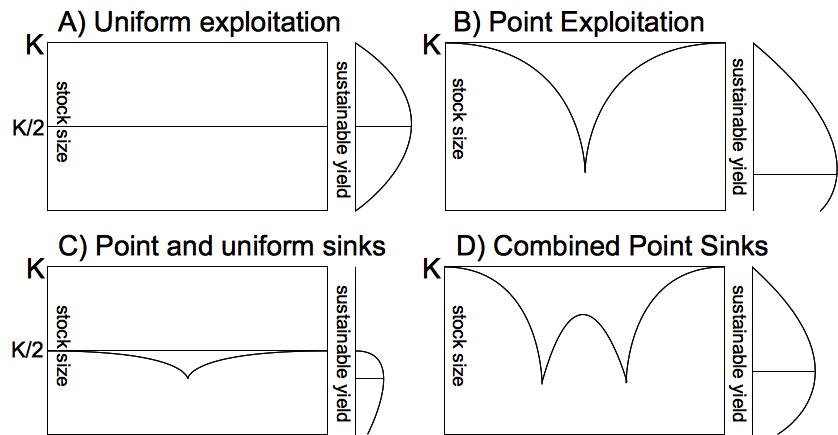
\includegraphics[width=6.5in]{capacity.png}
  \caption{Examples of distributed commons exploitation at maximum sustainable yield, and the associated yield graphs.  (A) shows uniform exploitation, with MSY at a stock size of half the carrying capacity.  (B) has a single point sink of exploitation: the total MSY is higher, since stocks are flowing in from neighboring regions; the MSY stock may be higher or lower depending on characteristics of the resource.  (C) shows a point sink under conditions where the total stock is already uniformly exploited: now both the maximum yield and the stock at that yield are much lower.  (D) shows the effect of multiple point sinks, with an intermediate region of much lower stocks.  In the extreme, the region between the two point sinks would be devoid of resources.}
  \label{fig:capacity}
\end{figure}

\section*{Leveraging Governance for a Distributed Commons}

% PART 2
% Capacity for local fishing communities to encourage regulatory regimes that then support their ability to self-organize sustainable fisheries.

Local fishing communities have born the greatest impact from fishery collapse.  While many communities historically developed commons management practices to maintain the resource sustainably the cross-border effects of the distributed fishery commons have undermined these regimes.  Research on Social-Ecological System (SES) commons helps explain why fishing communities have such a difficult time self-organizing sustainable regimes: Their communities are large and not well constrained and the stock is mobile and unpredictable \citep{ostrom2009general}.  These are exactly the reasons for modeling the resource as a distributed commons.

Further discussion and modeling of this situation requires that we focus on a particular central stakeholder.  For a fishing community that desires sustainable management (and knows what it entails by virtue of a historical tradition or hearing about another success), that desire can be said to have a ``nucleus''-- a core group with the capacity to deliberate on their situation.  Other members of the distributed commons are at a distance from that nucleus: some have a current fishing region which only partially overlaps; others have closer affiliations with outside nuclei.

% TODO: View from regional governance (food and export, protect or exploit, potential to close the commons)

From the government's perspective, the distributed details of the common may be less important.  Many users are encapsulated behind a single market, a single revenue stream, and an aggregate well-being. If the scope of the fishery is smaller than the scope of the government, the "outsiders" may be other national interests: corporate fishers, or impacts from agricultural or industrial sectors.

In the interests of maximizing well-being or tax revenue, the government's first priority is to maximizing the total sustainable (or the total economically sustainable, \citep{roughgarden1996fisheries}) catch.  Depending on the characteristics of the fish species, this requires a combination of gear restrictions (to protect vital life stages or supporting species), ITQs (or other restrictions on total catch), and Marine Protected Areas (to protect vital habitats).

% TODO: View from local fisheries (livelihood, but temporary; shifting baseline; potential for community management)
% TODO: View of outsiders: potential for exploitation, cross-border problems
 
From the perspective of the nucleus, the management concerns are different.  These include a reliable livelihood (through a social safety net), the elimination of outside drains, and support for self-management (served by closing borders).  Scientific information would also serve these goals, but the current animosity and distrust that many fishing communities have for the scientific community obstructs this avenue.

Two questions are critical for the nucleus.  The first is what changes in the conditions of access and usage would best support a better fishing regime.  The second is about methods for encouraging these changes.  I will not focus on the second question.  Options for it include campaigning, lobbying, or scientific support.

The research on SES commons has implications for the best options that an overarching governance body has for encouraging self-organization: for example, it can close the commons (through a quota system), or enforce boundaries on the commons (using a police force).  \citet{ostrom2009general} identifies the size of the resource system, its productivity, its predictability, the mobility of its units, the number of users, leadership, norms and social capital, knowledge, importance of the resource, and the ability to create rules as important factors determining the capacity of users to self-organize.

For classic commons, these ten factors determine whether the expected benefits of managing the commons exceed the perceived costs.  For a distributed commons, that result can differ in space, and the factors determine the scope of such management regimes.

% TODO: discuss the cross-boundary effects

% TODO:
% Include notes from wiki...
%
% Q's to address:
% How does this explain why fishermen are so dismissive of the potential for organizing for sustainable fisheries?
% Explain skepticism of scientific results
% Explain fighting against regional management - exploit or manage?
% Include discussion of stakeholders
% Include perverse incentives from regulation (e.g. lots of boats)
% Entities: small fisher, large fisher, outsider; local market, government, global market, scientists
% Multi-scale view: [ ... ] [ ... outsider ] [ [ships, fishing grounds] ] - gov and mgmt regions

\newpage
\singlespacing
\bibliography{paper}{}
\bibliographystyle{apalike}

\end{document}
